\documentclass[aspectratio=169, 11pt]{beamer}

% Theme and color scheme
\usetheme{Madrid}
\usecolortheme{default}

% Packages
\usepackage[utf8]{inputenc}
\usepackage[T1]{fontenc}
\usepackage{amsmath}
\usepackage{amsfonts}
\usepackage{amssymb}
\usepackage{graphicx}
\usepackage{booktabs}
\usepackage{xcolor}
\usepackage{tikz}
\usepackage{array}
\usepackage{multirow}
\usetikzlibrary{arrows.meta, positioning, shapes.geometric, backgrounds, fit}

% Color definitions
\definecolor{ulblue}{RGB}{214,214,240}  % #D6D6F0
\definecolor{ulgreen}{RGB}{102,153,51}
\definecolor{nercolor}{RGB}{230,126,34}
\definecolor{linkcolor}{RGB}{155,89,182}
\definecolor{relcolor}{RGB}{52,152,219}
\definecolor{graphcolor}{RGB}{46,125,50}

% Custom title page
\setbeamercolor{title page}{bg=ulblue}
\setbeamercolor{title}{fg=black}
\setbeamercolor{author}{fg=black}
\setbeamercolor{institute}{fg=black}
\setbeamercolor{date}{fg=black}
\setbeamerfont{title}{series=\bfseries,size=\Large}

% Header customization
\setbeamercolor{frametitle}{bg=ulblue,fg=black}
\setbeamercolor{block title}{bg=ulgreen,fg=white}

% Presentation information
\title{Transforming Unstructured Biomedical Text into Actionable Knowledge Graphs}
\subtitle{A Multi-Model Approach for Healthcare Information Extraction}
\author{Oyetunji Daniel \textsc{Abioye}}
\institute[UL]{
    \includegraphics[height=1cm]{assets/UL.png}\hspace{0.5cm}
    \includegraphics[height=1cm]{assets/IDMC.png}\\
    \textit{L'Institut des Sciences du Digital Management \& Cognition}\\
    \textit{Université de Lorraine}
}
\date{\today}

\begin{document}

% Title slide
\begin{frame}
    \usebeamercolor[bg]{title page}
    \setbeamercolor{background canvas}{bg=ulblue}
    \titlepage
\end{frame}

% Outline
\begin{frame}{Outline}
    \tableofcontents[hideallsubsections]
\end{frame}

\section{Introduction}

\begin{frame}{The Challenge: Unstructured Biomedical Data}
    \vspace{0.5cm}
    \begin{columns}[T]
        \begin{column}{0.6\textwidth}
            \begin{itemize}
                \setlength{\itemsep}{0.4cm}
                \item \textbf{80\% of biomedical data} is unstructured text
                \item Includes:
                \begin{itemize}
                    \setlength{\itemsep}{0.2cm}
                    \item Clinical notes and EHRs
                    \item Research publications (35M+ PubMed citations)
                    \item Case reports and protocols
                \end{itemize}
                \item Rich knowledge locked in narrative form
                \item Not directly usable by computers
            \end{itemize}
        \end{column}
        \begin{column}{0.4\textwidth}
            \centering
            \vspace{0.5cm}
            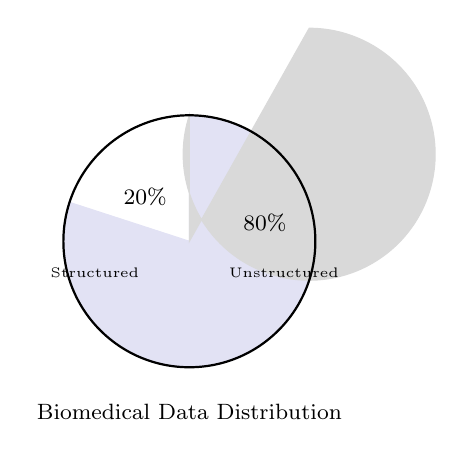
\begin{tikzpicture}[scale=0.8]
                % Manual pie chart - corrected for 80-20 split
                \filldraw[ulblue!70] (0,0) -- (0,2) arc (90:-198:2) -- cycle;
                \filldraw[gray!30] (0,0) -- (0,2) arc (-198:90:2) -- cycle;
                \draw[thick] (0,0) circle (2);
                
                \node at (1.2,0.3) {\footnotesize 80\%};
                \node at (-0.7,0.7) {\footnotesize 20\%};
                \node at (-1.5,-0.5) {\tiny Structured};
                \node at (1.5,-0.5) {\tiny Unstructured};
                \node at (0,-2.7) {\footnotesize Biomedical Data Distribution};
            \end{tikzpicture}
        \end{column}
    \end{columns}
\end{frame}

\begin{frame}{From Text to Knowledge}
    \vspace{0.8cm}
    \begin{center}
        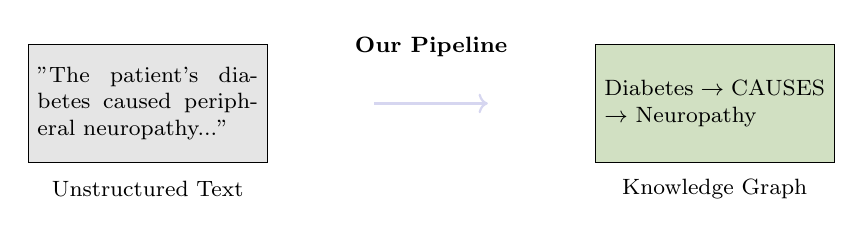
\begin{tikzpicture}[scale=0.9]
            \node[draw, rectangle, fill=gray!20, minimum width=3cm, minimum height=1.5cm] (text) at (0,0) {
                \begin{minipage}{2.8cm}
                    \footnotesize
                    "The patient's diabetes caused peripheral neuropathy..."
                \end{minipage}
            };
            
            \node[draw, rectangle, fill=ulgreen!30, minimum width=3cm, minimum height=1.5cm] (kg) at (8,0) {
                \begin{minipage}{2.8cm}
                    \footnotesize
                    Diabetes $\rightarrow$ CAUSES $\rightarrow$ Neuropathy
                \end{minipage}
            };
            
            \draw[->, thick, ulblue] (3.2,0) -- (4.8,0);
            \node at (4,0.8) {\footnotesize \textbf{Our Pipeline}};
            
            \node at (0,-1.2) {\footnotesize Unstructured Text};
            \node at (8,-1.2) {\footnotesize Knowledge Graph};
        \end{tikzpicture}
    \end{center}
    
    \vspace{0.8cm}
    \begin{block}{Research Question}
        \textbf{How can unstructured biomedical text be transformed into an actionable knowledge graph using a multi-model approach for information extraction?}
    \end{block}
\end{frame}

\begin{frame}{Research Objectives}
    \vspace{0.5cm}
    \begin{enumerate}
        \setlength{\itemsep}{0.6cm}
        \item \textbf{Design and implement} a multi-model NLP pipeline for biomedical text
        
        \item \textbf{Compare domain-specific vs. general language models} for relationship extraction
        
        \item \textbf{Construct an actionable biomedical knowledge graph} using Neo4j
        
        \item \textbf{Ensure ethical compliance} with data usage policies
        
        \item \textbf{Evaluate performance} using precision, recall, and F1 metrics
    \end{enumerate}
\end{frame}

\section{Background \& Motivation}

\begin{frame}{Why Knowledge Graphs for Biomedicine?}
    \vspace{0.3cm}
    \begin{columns}[T]
        \begin{column}{0.5\textwidth}
            \textbf{Natural Representation:}
            \begin{itemize}
                \setlength{\itemsep}{0.3cm}
                \item Entities: genes, diseases, drugs
                \item Relationships: treats, causes, affects
                \item Preserves complex interactions
            \end{itemize}
            
            \vspace{0.5cm}
            \textbf{Enables:}
            \begin{itemize}
                \setlength{\itemsep}{0.3cm}
                \item Knowledge discovery
                \item Complex queries
                \item Drug repurposing
                \item Hypothesis generation
            \end{itemize}
        \end{column}
        \begin{column}{0.5\textwidth}
            \centering
            \vspace{1cm}
            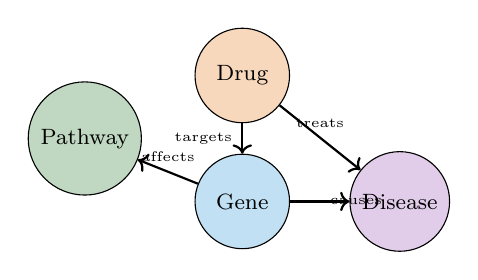
\begin{tikzpicture}[scale=0.8]
                \node[circle, draw, fill=nercolor!30, minimum size=1.2cm] (drug) at (0,2) {\footnotesize Drug};
                \node[circle, draw, fill=linkcolor!30, minimum size=1.2cm] (disease) at (2.5,0) {\footnotesize Disease};
                \node[circle, draw, fill=relcolor!30, minimum size=1.2cm] (gene) at (0,0) {\footnotesize Gene};
                \node[circle, draw, fill=graphcolor!30, minimum size=1.2cm] (pathway) at (-2.5,1) {\footnotesize Pathway};
                
                \draw[->, thick] (drug) -- node[above] {\tiny treats} (disease);
                \draw[->, thick] (gene) -- node[right] {\tiny causes} (disease);
                \draw[->, thick] (drug) -- node[left] {\tiny targets} (gene);
                \draw[->, thick] (gene) -- node[above] {\tiny affects} (pathway);
            \end{tikzpicture}
        \end{column}
    \end{columns}
\end{frame}

\begin{frame}{Current Challenges in Biomedical NLP}
    \vspace{0.3cm}
    \begin{block}{Unstructured Text Challenges}
        \begin{itemize}
            \setlength{\itemsep}{0.3cm}
            \item Domain-specific terminology and abbreviations
            \item Variable nomenclature across contexts
            \item Complex sentence structures
            \item Context-dependent meanings
        \end{itemize}
    \end{block}
    
    \vspace{0.4cm}
    \begin{block}{Scale and Integration Issues}
        \begin{itemize}
            \setlength{\itemsep}{0.3cm}
            \item Exponential growth: thousands of papers daily
            \item Heterogeneous data sources
            \item Quality inconsistencies
            \item Integration complexity
        \end{itemize}
    \end{block}
\end{frame}

\section{Literature Review}

\begin{frame}{Evolution of Biomedical NLP}
    \vspace{0.5cm}
    \centering
    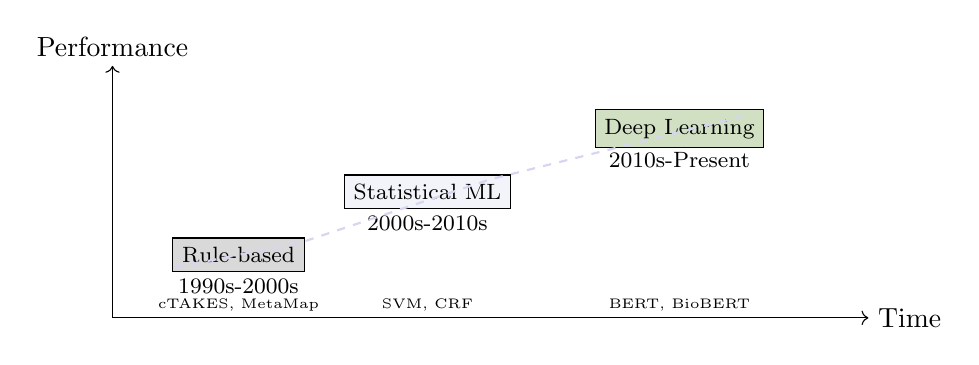
\begin{tikzpicture}[scale=0.8]
        \draw[->] (0,0) -- (12,0) node[right] {Time};
        \draw[->] (0,0) -- (0,4) node[above] {Performance};
        
        \node at (2,0.5) {\footnotesize 1990s-2000s};
        \node at (2,1) [rectangle, draw, fill=gray!30] {\footnotesize Rule-based};
        \node at (2,0.2) {\tiny cTAKES, MetaMap};
        
        \node at (5,1.5) {\footnotesize 2000s-2010s};
        \node at (5,2) [rectangle, draw, fill=ulblue!30] {\footnotesize Statistical ML};
        \node at (5,0.2) {\tiny SVM, CRF};
        
        \node at (9,2.5) {\footnotesize 2010s-Present};
        \node at (9,3) [rectangle, draw, fill=ulgreen!30] {\footnotesize Deep Learning};
        \node at (9,0.2) {\tiny BERT, BioBERT};
        
        \draw[dashed, thick, ulblue] (1,0.8) -- (3,1.2) -- (6,2.2) -- (10,3.2);
    \end{tikzpicture}
    
    \vspace{0.8cm}
    \begin{itemize}
        \setlength{\itemsep}{0.4cm}
        \item \textbf{Rule-based} → \textbf{Statistical ML} → \textbf{Transformer-based}
        \item Domain-specific models: BioBERT, ClinicalBERT, SciBERT
        \item Latest: Large Language Models (GPT, Gemma, MedGemma)
    \end{itemize}
\end{frame}

\begin{frame}{State-of-the-Art Approaches}
    \vspace{0.3cm}
    \begin{columns}[T]
        \begin{column}{0.5\textwidth}
            \textbf{Named Entity Recognition:}
            \begin{itemize}
                \setlength{\itemsep}{0.2cm}
                \item GLiNER: Zero-shot, lightweight
                \item Natural language descriptors
                \item 6\% F1 improvement over previous systems
            \end{itemize}
            
            \vspace{0.4cm}
            \textbf{Entity Linking:}
            \begin{itemize}
                \setlength{\itemsep}{0.2cm}
                \item UMLS: 3M+ medical concepts
                \item SciSpacy: TF-IDF character n-grams
                \item Handles abbreviations and synonyms
            \end{itemize}
        \end{column}
        \begin{column}{0.5\textwidth}
            \textbf{Relationship Extraction:}
            \begin{itemize}
                \setlength{\itemsep}{0.2cm}
                \item Rule-based → ML → Neural → LLMs
                \item Zero-shot with prompting
                \item Domain-specific vs. general models
            \end{itemize}
            
            \vspace{0.4cm}
            \textbf{Knowledge Graphs:}
            \begin{itemize}
                \setlength{\itemsep}{0.2cm}
                \item Neo4j property graphs
                \item Cypher query language
                \item Scalable graph traversal
            \end{itemize}
        \end{column}
    \end{columns}
\end{frame}

\section{Methodology}

\begin{frame}{System Architecture Overview}
    \vspace{0.5cm}
    \begin{center}
        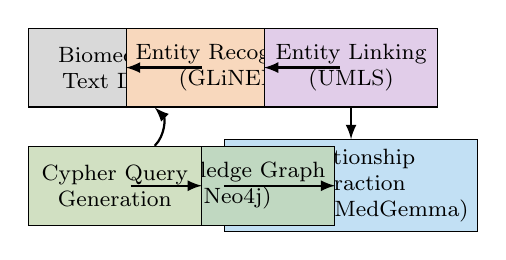
\begin{tikzpicture}[
            node distance=1.5cm,
            block/.style={rectangle, draw, fill=blue!20, minimum width=2.2cm, minimum height=1cm, font=\footnotesize, align=center},
            arrow/.style={->, >=latex, thick}
        ]
            \node[block, fill=gray!30] (data) {Biomedical\\Text Data};
            \node[block, right of=data, fill=nercolor!30] (ner) {Entity Recognition\\(GLiNER)};
            \node[block, right of=ner, fill=linkcolor!30] (linking) {Entity Linking\\(UMLS)};
            \node[block, below of=linking, fill=relcolor!30] (relation) {Relationship\\Extraction\\(Gemma/MedGemma)};
            \node[block, left of=relation, fill=graphcolor!30] (graph) {Knowledge Graph\\(Neo4j)};
            \node[block, left of=graph, fill=ulgreen!30] (cypher) {Cypher Query\\Generation};
            
            \draw[arrow] (data) -- (ner);
            \draw[arrow] (ner) -- (linking);
            \draw[arrow] (linking) -- (relation);
            \draw[arrow] (relation) -- (graph);
            \draw[arrow] (graph) -- (cypher);
            \draw[arrow, bend right=45] (cypher) to (data);
        \end{tikzpicture}
    \end{center}
    
    \vspace{0.6cm}
    \textbf{Modular Pipeline:} Each component can be independently optimized and replaced
\end{frame}

\begin{frame}{Component 1: Named Entity Recognition}
    \vspace{0.3cm}
    \begin{columns}[T]
        \begin{column}{0.5\textwidth}
            \textbf{GLiNER-BioMed:}
            \begin{itemize}
                \setlength{\itemsep}{0.2cm}
                \item Zero-shot NER capability
                \item Natural language entity descriptions
                \item Lightweight and efficient
                \item Configurable confidence thresholds
            \end{itemize}
            
            \vspace{0.4cm}
            \textbf{Entity Types:}
            \begin{itemize}
                \setlength{\itemsep}{0.2cm}
                \item Problems/Conditions
                \item Treatments/Drugs
                \item Tests/Procedures
                \item Species, Variants
            \end{itemize}
        \end{column}
        \begin{column}{0.5\textwidth}
            \vspace{0.5cm}
            \begin{exampleblock}{Example}
                \footnotesize
                \textbf{Input:} "The patient was started on metformin for diabetes mellitus."
                
                \textbf{Output:}
                \begin{itemize}
                    \item \textcolor{nercolor}{"metformin"} → Drug
                    \item \textcolor{linkcolor}{"diabetes mellitus"} → Condition
                \end{itemize}
            \end{exampleblock}
        \end{column}
    \end{columns}
\end{frame}

\begin{frame}{Component 2: Entity Linking to UMLS}
    \vspace{0.3cm}
    \begin{columns}[T]
        \begin{column}{0.5\textwidth}
            \textbf{SciSpacy UMLS Linker:}
            \begin{itemize}
                \setlength{\itemsep}{0.2cm}
                \item TF-IDF character n-gram matching
                \item 3+ million UMLS concepts
                \item Similarity threshold: 0.7
                \item Abbreviation resolution
            \end{itemize}
            
            \vspace{0.4cm}
            \textbf{Benefits:}
            \begin{itemize}
                \setlength{\itemsep}{0.2cm}
                \item Canonical identifiers (CUIs)
                \item Synonym consolidation
                \item Interoperability
            \end{itemize}
        \end{column}
        \begin{column}{0.5\textwidth}
            \vspace{0.3cm}
            \begin{exampleblock}{Linking Example}
                \footnotesize
                \textbf{Entity:} "metformin"
                
                \textbf{UMLS Link:}
                \begin{itemize}
                    \item CUI: C0025598
                    \item Name: "Metformin"
                    \item Similarity: 0.98
                    \item Semantic Type: Drug
                \end{itemize}
            \end{exampleblock}
            
            \vspace{0.4cm}
            Same concept ID for synonyms:
            \begin{itemize}
                \setlength{\itemsep}{0.1cm}
                \item "heart attack" → C0027051
                \item "myocardial infarction" → C0027051
            \end{itemize}
        \end{column}
    \end{columns}
\end{frame}

\begin{frame}{Component 3: Relationship Extraction}
    \begin{columns}
        \begin{column}{0.5\textwidth}
            \textbf{Model Comparison:}
            \begin{itemize}
                \item \textcolor{ulblue}{Gemma-3-4b-it}: General-purpose
                \item \textcolor{ulgreen}{MedGemma-3-4b}: Medical domain-specific
            \end{itemize}
            
            \textbf{Prompt Strategies:}
            \begin{itemize}
                \item Basic: Simple task description
                \item Few-shot: 2-3 examples
                \item Structured: Detailed format requirements
            \end{itemize}
        \end{column}
        \begin{column}{0.5\textwidth}
            \begin{exampleblock}{Prompt Example}
                \footnotesize
                \textbf{Task:} Extract relationships as (Entity1, Relation, Entity2)
                
                \textbf{Text:} "diabetes caused peripheral neuropathy"
                
                \textbf{Expected:} (diabetes, causes, peripheral neuropathy)
            \end{exampleblock}
        \end{column}
    \end{columns}
    
    \vspace{0.5cm}
    \textbf{Output Validation:} Entity matching, relation validation, deduplication
\end{frame}

\begin{frame}{Component 4: Neo4j Knowledge Graph}
    \begin{columns}
        \begin{column}{0.5\textwidth}
            \textbf{Graph Schema:}
            \begin{itemize}
                \item Nodes: \texttt{:MedicalEntity}
                \item Properties: CUI, name, semantic type
                \item Relationships: CAUSES, TREATS, etc.
                \item Provenance: source document info
            \end{itemize}
            
            \textbf{Cypher Generation:}
            \begin{itemize}
                \item Automated query creation
                \item MERGE operations (avoid duplicates)
                \item Batch processing for efficiency
            \end{itemize}
        \end{column}
        \begin{column}{0.5\textwidth}
            \begin{exampleblock}{Cypher Example}
                \footnotesize
                \texttt{MERGE (a:MedicalEntity \\
                \hspace{1cm}\{cui:"C0011849"\})\\
                ON CREATE SET a.name = "Diabetes"\\[0.3cm]
                MERGE (b:MedicalEntity \\
                \hspace{1cm}\{cui:"C0031117"\})\\
                ON CREATE SET b.name = "Neuropathy"\\[0.3cm]
                MERGE (a)-[:CAUSES]->(b)}
            \end{exampleblock}
        \end{column}
    \end{columns}
\end{frame}

\section{Evaluation Setup}

\begin{frame}{BioRED Dataset}
    \vspace{0.3cm}
    \begin{columns}[T]
        \begin{column}{0.6\textwidth}
            \textbf{Dataset Characteristics:}
            \begin{itemize}
                \setlength{\itemsep}{0.2cm}
                \item 600 annotated PubMed abstracts
                \item 20,000+ entity mentions
                \item 6,000+ relationship annotations
                \item 6 entity types, 8 relation types
            \end{itemize}
            
            \vspace{0.4cm}
            \textbf{Entity Types:}
            \begin{itemize}
                \setlength{\itemsep}{0.15cm}
                \item GeneOrGeneProduct
                \item DiseaseOrPhenotypicFeature
                \item ChemicalEntity
                \item SequenceVariant, CellLine, OrganismTaxon
            \end{itemize}
        \end{column}
        \begin{column}{0.4\textwidth}
            \textbf{Relation Types:}
            \begin{itemize}
                \setlength{\itemsep}{0.15cm}
                \item Association
                \item Positive\_Correlation
                \item Negative\_Correlation
                \item Bind
                \item Comparison
                \item Cotreatment
                \item Drug\_Interaction
                \item Conversion
            \end{itemize}
        \end{column}
    \end{columns}
    
    \vspace{0.6cm}
    \textbf{Evaluation Metrics:} Precision, Recall, F1-score with exact, partial, and text-based matching
\end{frame}

\begin{frame}{Model Configurations}
    \vspace{0.5cm}
    \begin{table}[h]
        \centering
        \footnotesize
        \begin{tabular}{|l|l|l|}
        \hline
        \textbf{Component} & \textbf{Model/Method} & \textbf{Configurations} \\
        \hline
        NER & GLiNER-BioMed & Thresholds: 0.3, 0.5, 0.7 \\
        \hline
        Entity Linking & SciSpacy UMLS & Similarity threshold: 0.7 \\
        \hline
        \multirow{2}{*}{Relation Extraction} & Gemma-3-4b-it & Basic, Few-shot, Structured \\
        \cline{2-3}
         & MedGemma-3-4b & Basic, Few-shot, Structured \\
        \hline
        Knowledge Graph & Neo4j & Property graph model \\
        \hline
        \end{tabular}
    \end{table}
    
    \vspace{0.6cm}
    \textbf{Experimental Matrix:} 6 relationship extraction configurations (2 models × 3 prompting strategies)
\end{frame}

\section{Results \& Analysis}

\begin{frame}{Named Entity Recognition Results}
    \vspace{0.3cm}
    \begin{table}[h]
        \centering
        \footnotesize
        \caption{GLiNER-BioMed Performance Across Configurations}
        \begin{tabular}{llccc}
        \toprule
        \textbf{Threshold} & \textbf{Matching} & \textbf{F1} & \textbf{Precision} & \textbf{Recall} \\
        \midrule
        \textcolor{ulgreen}{Low (0.3)} & \textcolor{ulgreen}{Partial} & \textcolor{ulgreen}{\textbf{0.447}} & 0.620 & 0.349 \\
        Low (0.3) & Exact & 0.400 & 0.555 & 0.313 \\
        Default (0.5) & Partial & 0.336 & 0.694 & 0.221 \\
        Default (0.5) & Exact & 0.302 & 0.624 & 0.199 \\
        High (0.7) & Partial & 0.164 & 0.755 & 0.092 \\
        High (0.7) & Exact & 0.152 & 0.699 & 0.085 \\
        \bottomrule
        \end{tabular}
    \end{table}
    
    \vspace{0.4cm}
    \textbf{Key Findings:}
    \begin{itemize}
        \setlength{\itemsep}{0.2cm}
        \item Best performance: Low threshold + Partial matching (F1: 0.447)
        \item Conservative behavior: High precision, limited recall
        \item Boundary detection challenges (partial > exact matching)
    \end{itemize}
\end{frame}

\begin{frame}{Relationship Extraction: Gemma vs MedGemma}
    \vspace{0.3cm}
    \begin{table}[h]
        \centering
        \footnotesize
        \caption{Relationship Extraction Performance Comparison}
        \begin{tabular}{llcc}
        \toprule
        \textbf{Model} & \textbf{Strategy} & \textbf{F1} & \textbf{Precision/Recall} \\
        \midrule
        \textcolor{ulblue}{Gemma} & \textcolor{ulblue}{Few-shot} & \textcolor{ulblue}{\textbf{0.082}} & 0.082 / 0.082 \\
        Gemma & Basic & 0.073 & 0.073 / 0.073 \\
        MedGemma & Few-shot & 0.070 & 0.087 / 0.059 \\
        Gemma & Structured & 0.069 & 0.075 / 0.065 \\
        MedGemma & Basic & 0.063 & 0.084 / 0.050 \\
        MedGemma & Structured & 0.053 & 0.068 / 0.043 \\
        \bottomrule
        \end{tabular}
    \end{table}
    
    \vspace{0.4cm}
    \textbf{Surprising Findings:}
    \begin{itemize}
        \setlength{\itemsep}{0.3cm}
        \item \textcolor{ulblue}{General Gemma outperformed domain-specific MedGemma}
        \item Few-shot prompting most effective across both models
        \item Overall low F1 scores (5-8\%) indicate task difficulty
    \end{itemize}
\end{frame}

\begin{frame}{Key Finding: General vs Domain-Specific Models}
    \vspace{0.4cm}
    \begin{columns}[T]
        \begin{column}{0.5\textwidth}
            \textbf{Gemma (General):}
            \begin{itemize}
                \setlength{\itemsep}{0.3cm}
                \item Higher recall (8.2\%)
                \item Balanced precision-recall
                \item Better overall F1 scores
                \item More liberal relationship detection
            \end{itemize}
        \end{column}
        \begin{column}{0.5\textwidth}
            \textbf{MedGemma (Domain-specific):}
            \begin{itemize}
                \setlength{\itemsep}{0.3cm}
                \item Higher precision (8.7\%)
                \item Lower recall (5.9\%)
                \item More conservative predictions
                \item Medical domain knowledge may be limiting
            \end{itemize}
        \end{column}
    \end{columns}
    
    \vspace{0.6cm}
    \begin{alertblock}{Counterintuitive Result}
        Domain specialization did not improve relationship extraction performance. General language understanding may be more valuable than medical-specific training for complex biomedical relationship identification.
    \end{alertblock}
\end{frame}

\begin{frame}{Performance Challenges \& Limitations}
    \begin{block}{Relationship Extraction Challenges}
        \begin{itemize}
            \item \textbf{Low F1 scores (5-8\%)} across all configurations
            \item Model size constraint: 4B parameters vs. state-of-the-art 70B+
            \item Output formatting inconsistencies
            \item Entity alignment problems
            \item Hallucination and inference issues
        \end{itemize}
    \end{block}
    
    \begin{block}{NER Limitations}
        \begin{itemize}
            \item Conservative recall (20-35\%)
            \item Boundary detection challenges
            \item Context sensitivity issues
            \item Missing uncommon terms and new expressions
        \end{itemize}
    \end{block}
    
    \textbf{Impact:} Limited recall propagates through pipeline, affecting knowledge graph completeness
\end{frame}

\section{Discussion}

\begin{frame}{Clinical Applicability \& Architecture Strengths}
    \begin{columns}
        \begin{column}{0.5\textwidth}
            \textbf{Current Limitations:}
            \begin{itemize}
                \item Performance too low for critical clinical applications
                \item High-precision, low-recall characteristics
                \item Requires significant improvement for deployment
            \end{itemize}
            
            \textbf{Potential Applications:}
            \begin{itemize}
                \item Literature screening (high precision)
                \item Knowledge base enrichment
                \item Hypothesis generation starting points
            \end{itemize}
        \end{column}
        \begin{column}{0.5\textwidth}
            \textbf{Technical Strengths:}
            \begin{itemize}
                \item \textcolor{ulgreen}{Modular architecture}
                \item \textcolor{ulblue}{UMLS integration} for interoperability
                \item \textcolor{nercolor}{Flexible configuration} options
                \item \textcolor{graphcolor}{Scalable Neo4j} backend
            \end{itemize}
            
            \textbf{Foundation for Future Work:}
            \begin{itemize}
                \item Easy component replacement
                \item Independent optimization
                \item Standards-based approach
            \end{itemize}
        \end{column}
    \end{columns}
\end{frame}

\section{Conclusions \& Future Work}

\begin{frame}{Key Contributions}
    \vspace{0.2cm}
    \begin{block}{Technical Contributions}
        \begin{itemize}
            \setlength{\itemsep}{0.2cm}
            \item \textbf{Multi-model pipeline} integrating GLiNER, SciSpacy, and LLMs
            \item \textbf{Scalable graph construction} with efficient Cypher generation
            \item \textbf{Comprehensive evaluation framework} using BioRED dataset
        \end{itemize}
    \end{block}
    
    \vspace{0.3cm}
    \begin{block}{Theoretical Contributions}
        \begin{itemize}
            \setlength{\itemsep}{0.2cm}
            \item \textbf{Domain specialization analysis}: General models outperformed medical-specific ones
            \item \textbf{Knowledge graph integration paradigm} for biomedical knowledge discovery
            \item \textbf{Multi-model approach} demonstrating end-to-end biomedical text transformation
        \end{itemize}
    \end{block}
\end{frame}

\begin{frame}{Future Research Directions}
    \vspace{0.2cm}
    \begin{enumerate}
        \setlength{\itemsep}{0.4cm}
        \item \textbf{Model Scale Improvements}
        \begin{itemize}
            \setlength{\itemsep}{0.1cm}
            \item Deploy larger language models (70B+ parameters)
            \item Specialized fine-tuning for biomedical relation extraction
        \end{itemize}
        
        \item \textbf{Multiple Knowledge Base Integration}
        \begin{itemize}
            \setlength{\itemsep}{0.1cm}
            \item Gene Ontology (GO), ChEBI, Human Phenotype Ontology
            \item Cross-ontology relationship discovery
        \end{itemize}
        
        \item \textbf{Pipeline Enhancements}
        \begin{itemize}
            \setlength{\itemsep}{0.1cm}
            \item Hybrid approaches combining rule-based and neural methods
            \item Context-aware entity recognition
            \item Improved confidence scoring mechanisms
        \end{itemize}
        
        \item \textbf{Real-world Deployment}
        \begin{itemize}
            \setlength{\itemsep}{0.1cm}
            \item Clinical decision support integration
            \item Large-scale literature processing
            \item Interactive knowledge discovery tools
        \end{itemize}
    \end{enumerate}
\end{frame}

\begin{frame}[plain]
    \begin{center}
        \Huge \textcolor{ulblue}{Thank You}
        
        \vspace{1cm}
        
        \Large Questions \& Discussion
        
        \vspace{1.5cm}
        
        \begin{tikzpicture}
            \node at (0,0) {\includegraphics[height=1.5cm]{assets/UL.png}};
            \node at (6,0) {\includegraphics[height=1.5cm]{assets/IDMC.png}};
        \end{tikzpicture}
        
        \vspace{0.5cm}
        
        \normalsize
        Oyetunji Daniel \textsc{Abioye}\\
        \textit{Supervised by: Maziyar \textsc{Panahi}}
    \end{center}
\end{frame}

\end{document}